Consider the radiation data (with door closed) in Example 4.10. Construct a \textit{Q-Q} plot
for the natural logarithms of these data. [Note that the natural logarithm transformation
corresponds to the value $\lambda = 0$ in (4--34).] Do the natural logarithms appear to be normally
distributed? Compare your results with Figure 4.13. Does the choice $\lambda = \frac{1}{4}$ or
$\lambda = 0$ make much difference in this case?

\begin{figure}[H]
    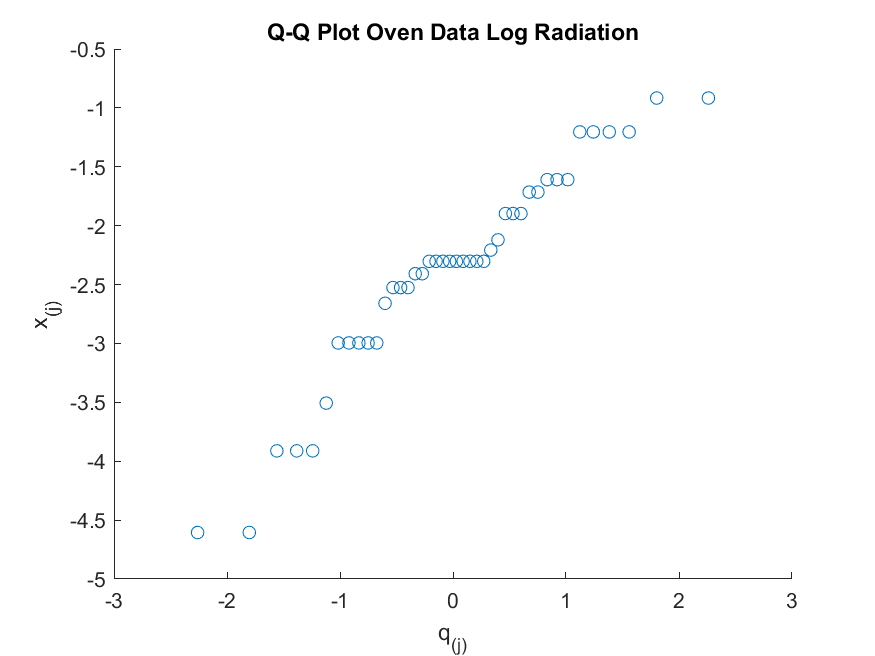
\includegraphics[scale=0.8]{./matlab/chapter-4/sol4.27.png}
\end{figure}

The Q-Q plot of the natural log transformed data does appear to be linear, so the data would be considered normally distributed after transformation. The plot here, when $\lambda = 0$, looks very similar to the one in Figure 4.13 when $\lambda = \frac{1}{4}$. The plot when $\lambda = \frac{1}{4}$ stretches things verically slightly compared to the log-transformation. I'd guess that either $\lambda$ value is a fine choice.